\begin{problem}%
{Робот}%
{\textsl{стандартный ввод}}%
{\textsl{стандартный вывод}}%
{2 секунды}%
{64 мегабайта}{}

Робот движется по полю, которое состоит из $N$ клеток, выстроенных в ряд. На каждой из клеток находится кубик определенного цвета.\\

До начала движения робот находится на первой клетке поля и не держит ни одного кубика. Находясь на клетке, робот может выполнить не более одного раза каждую из следующих операций: (1) положить кубик того же цвета, который лежит на текущей клетке; (2) поднять с клетки тот кубик, который находился там сначала. После этого робот перемещается на следующую клетку или останавливается, если текущая клетка последняя в поле.\\

Одновременно робот может держать не более $K$ кубиков. На момент остановки робот не должен держать ни одного кубика.\\

Напишите программу, которая по информации о цвете кубиков и ограничении на количество кубиков, которое может держать робот, определяет максимальное общее количество кубиков, которое робот может перенести с места на место, двигаясь по полю.

\InputFile

Первая строка входного файла содержит символьную строку длинны $N$ ($1 \le N \le 1000$). Строка состоит из маленьких букв латинского алфавита. Каждая буква соответствует клетке поля и определяет цвет кубика, который находится в этой клетке. Вторая строка содержит ограничение на количество кубиков, которое одновременно может держать робот $K$ ($1 \le K \le 25$).

\OutputFile

Единственная строка выходного файла должна содержать целое число — максимальное количество кубиков, месторасположение которых робот может изменить, двигаясь по полю.

\Examples

\begin{example}
\exmp{
rgbbggrmcm
2
}{%
4
}%
\end{example}

\Explanation

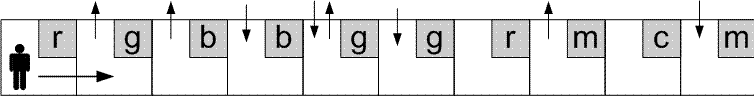
\includegraphics[scale=0.5]{images/1359.png}

\end{problem}